\documentclass{article}
\usepackage{amsmath, fullpage}
\usepackage[portuguese]{babel}
\usepackage{graphicx}
\usepackage{color}
\usepackage{subcaption}
\graphicspath{{imgs/}}


\begin{document}

\title{Memórias}
\author{Henrique Bernardes}
%\date{\vspace{-5ex}}
\maketitle
\thispagestyle{empty}
\section{Introdução - Registradores}
De início, temos os registradores, compostos por flip-flops e multiplexadores 2 para 1 controlados a partir de um sinal de "load":

\begin{figure}[h!] 
    \centering 
    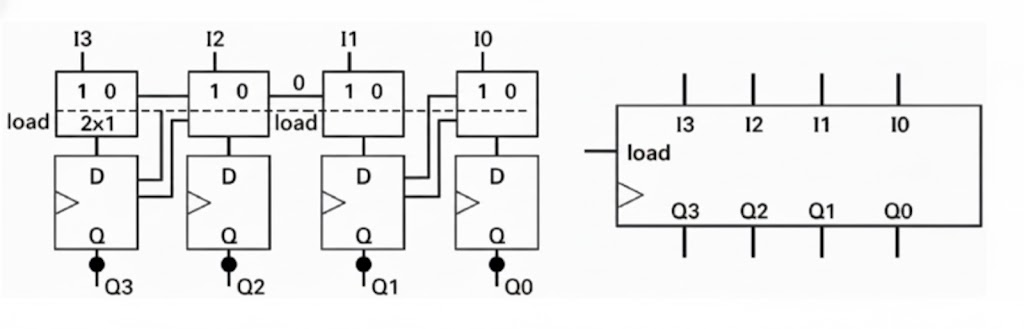
\includegraphics[width=0.8\textwidth]{registradores.jpg} 
    \caption{Registradores} 
    \label{fig:registradores} 
\end{figure}

Existem, aqui, duas situações:
\begin{itemize}
     \item Quando $ load = 1$ e $clk$ estiver na borda se subida, o flip-flop é carregado com a entrada de dados I ($I_i$)

     \item Quando $load = 0$ e $clk$ estiver na borda de subida, o flip-flop é carregado com sua saída Q ($Q_i$)
\end{itemize}


Essas estruturas simples podem ser utilizadas para criar os chamados "bancos de registradores". Os bancos de registradores utilizam endereços para acessar cada registrador. No exemplo da imagem \ref{fig:bancoderegistradores}, um decodificador 3:8 é utilizado para endereçar, a partir de 3 bits, 8 endereços e, então, direcionar o dado $input$ para o registrador adequado.

\begin{figure}[h!] 
    \centering 
    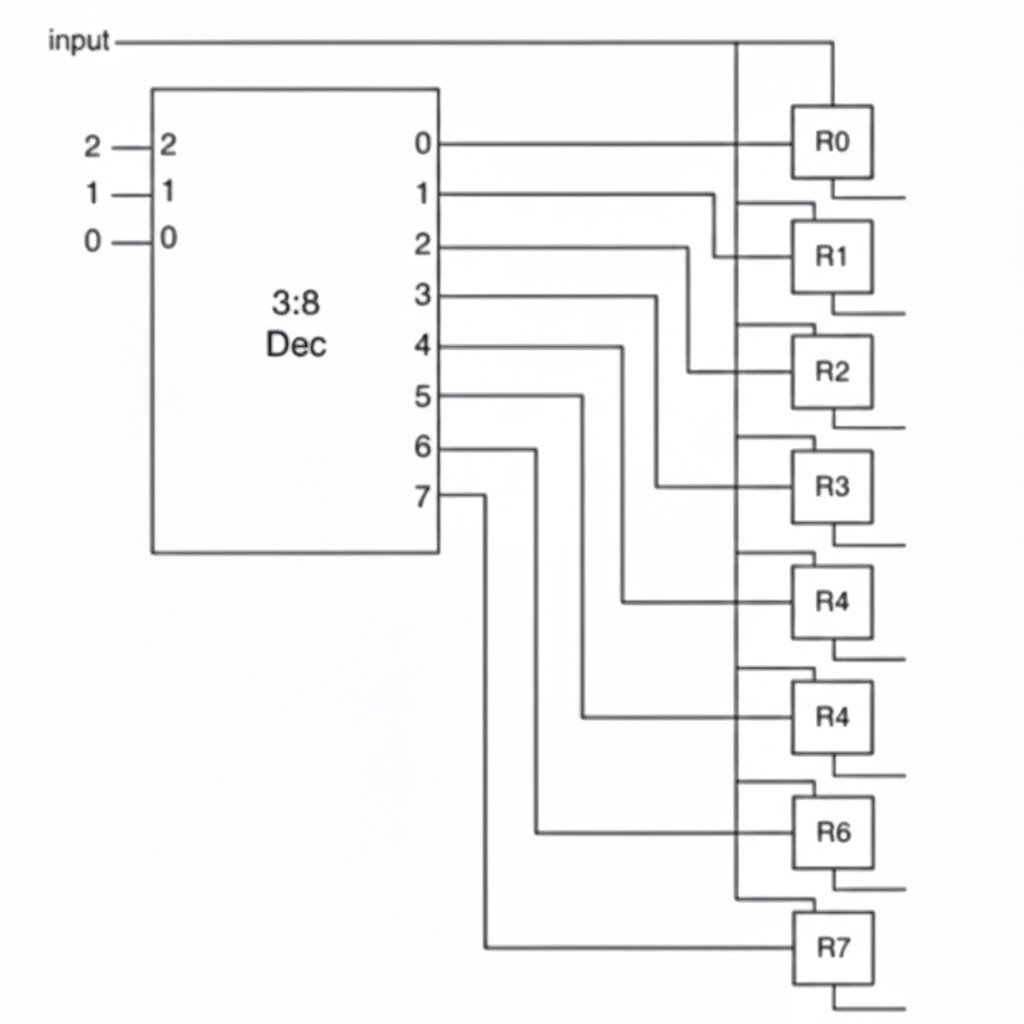
\includegraphics[width=0.2\textwidth]{bancoderegistradores.jpg} %
    \caption{Banco de Registradores} 
    \label{fig:bancoderegistradores} 
\end{figure}

\section{Memórias}


Em um projeto RTL, são utilizados componentes adicionais além dos blocos operacional e de controle, como por exemplo memórias. Um dos tipos de memória é denominada \textit{RAM - Random Access Memory}.

Como visto na imagem \ref{fig:ram}, um bloco de memória $RAM$ é descrito por dois números, como, na imagem, $1024x32$. O primeiro número, $1024$, indica o número de palavras(profundidade) que compõem o bloco de memória. Já o segundo número, $32$, indica o tamanho de cada palavra(largura). Cada palavra pode ser entendida como um registrador, ou seja, cada palavra pode ser lida e escrita individualmente a partir de entradas de endereço e dados. Detalhando os demais sinais:

\begin{itemize}
     \item $addr$ - 10 bits ($2^{10} = 1024$ palavras)
     \item $rw = 0$ - leitura
     \item $rw = 1$ - escrita
     \item $en = 0$ - desabilita a memória
\end{itemize}

Para realizar uma leitura, lê-se primeiro uma linha inteira de palavras e, então, seleciona-se a palavra apropriada nessa linha.

Finalmente, para armazenar uma maior quantidade de bits, uma $RAM$ típica, ao invés de utilizar flip-flops, utiliza estruturam mais compactas.


\begin{figure}[h!] 
    \centering 
    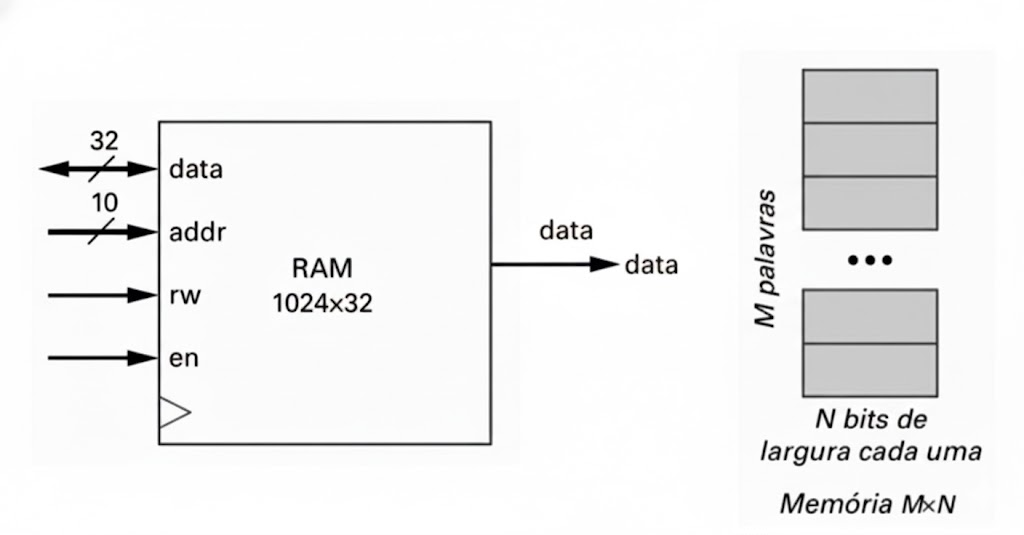
\includegraphics[width=0.7\textwidth]{RAM.jpg} %
    \caption{Memória RAM} 
    \label{fig:ram} 
\end{figure}


 
\subsection{Estrutura da RAM}

Uma $RAM$ se baseia em uma grade que contém blocos de armazenamento, ou as chamadas \textbf{células}. Cada célula é alimentada com um certo dado; contudo, apenas ao ser ativada pelo decodificado (de dimensão $AxM$), alimentado por um endereço, que as células dessa palavra específica são ativadas, como mostra a imagem \ref{fig:estruturaRam}.

\begin{figure}[h!] 
    \centering 
    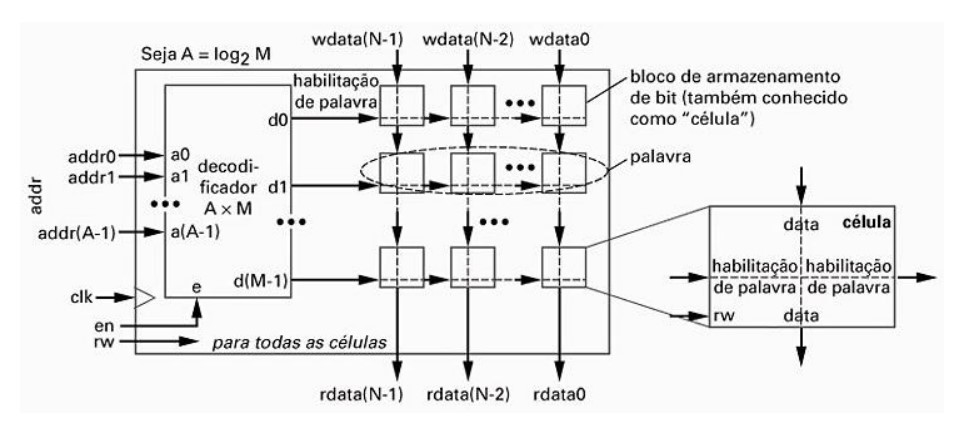
\includegraphics[width=0.7\textwidth]{estruturaRam.jpg}
    \caption{Estrutura da $RAM$, organizada em células que formam palavras na horizontal.} 
    \label{fig:estruturaRam} 
\end{figure}

A entrada $rw$ se conecta a todas as células e determina dois cenários para cada célula:
\begin{itemize}
     \item Se o valor da célula será lido e disponibilizado na saída $rdata(N-i)$
     \item Se o valor da entrada $wdata(N-i)$ será gravado na célula.
\end{itemize}

\section{Memória RAM estática(SRAM)}
No caso da SRAM, o bit fica armazenado no laço criado pelos inversores.

Para as operações de escrita:
\begin{itemize}
     \item Escrita de 1: Faz-se $data=1$ e $data'= 0$ e $enable = 1$, ativando os transistores.
     \item Escrita de 0: Faz-se $data=0$ e $data'= 1$ e $enable = 1$, ativando os transistores.
\end{itemize}


\begin{figure}[h]
\centering
\begin{minipage}{0.48\textwidth}
    \centering
    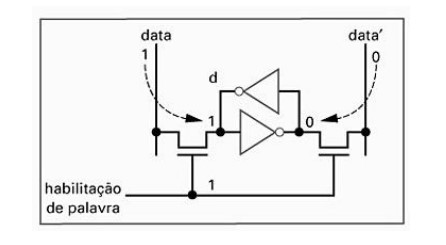
\includegraphics[width=\linewidth]{escritaSRam.jpg}
    \caption{Operação de escrita $SRAM$}
    \label{fig:escritaSRam}
\end{minipage}\hfill
\begin{minipage}{0.48\textwidth}
    \centering
    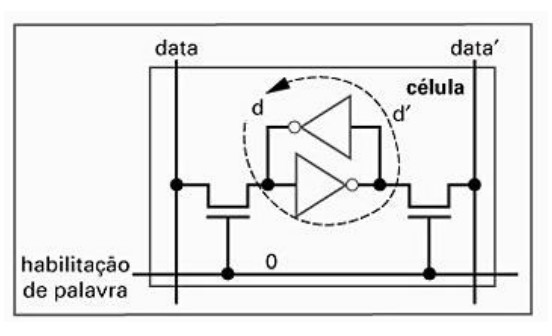
\includegraphics[width=\linewidth]{estruturaSRam.jpg}
    \caption{Estrutura $SRAM$, composta por seis transistores}
    \label{fig:estruturaSRam}
\end{minipage}
\end{figure}

Para as operações de leitura, primeiro se realiza o carregamento de $1$ em ambas as linhas $data$ e $data'$ e também no sinal de habilitação.

Em um dos lados, terá um $0$ armazenado, provocando uma queda de tensão. Um circuito amplificador e comparador de tensão detecta em qual lado houve a maior queda. 

\begin{itemize}
     \item Se a tensão em $data > data'$ então a célula tem $1$ armazenado. Houve queda de tensão em $data'$
     \item Se a tensão em $data < data'$ então a célula tem $0$ armazenado. Houve queda de tensão em $data$
\end{itemize}

Enquanto houver energia alimentando os transistores, a SRAM mantém o bit armazenado(volátil) sem que ele mude(estático).

Por ser composta de apenas seis transistores, a memória SRAM utiliza menos transistores que um flip-flop.

Por necessitar de um circuito amplificador e comparador, o acesso aos bits armazenados(leitura) requer mais tempo.
 
\begin{figure}[!h]
     \centering
     \def\svgwidth{0.5\textwidth}
     \input{imgs/sram1.eps_tex}
     \caption{\label{fig:img1} Estrutura interna da SRAM }
     \hfill
\end{figure}



\newpage

\section{Memória RAM Dinâmica(DRAM)}

A memória DRAM é composta por um capacitor e um transistor.


Para as operações de \textbf{escrita}, primeiro se escreve o valor a ser armazenado na linha $data$ e então $enable=1$, carregando o capacitor(de capacitância elevada) que, então, sofre uma lenta queda, como mostra a imagem \ref{fig:estruturaDRam}.


Para a operação de leitura, alimenta-se a linha de dados com uma tensão intermediaria entre $0$ e $1$. Depois, faz-se $enable=1$, fazendo com que a tensão armazenada no capacitor cause uma queda de tensão na linha de dados. Da mesma forma que na $SRAM$, aqui um circuito amplificador e comparador é utilizado para definir qual era o valor armazenado.
\begin{figure}[h!] 
    \centering 
    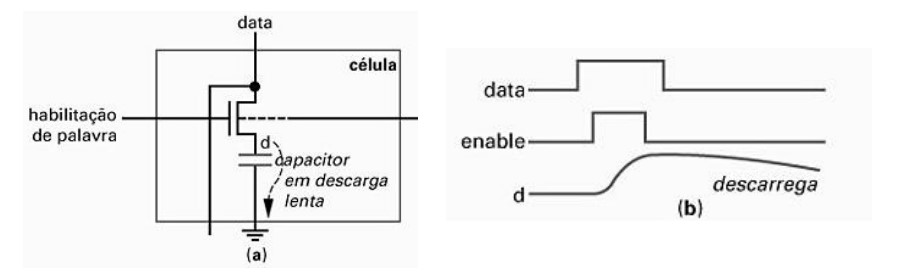
\includegraphics[width=1\textwidth]{estruturaDRam.jpg}
    \caption{Estrutura da $DRAM$, composta de um transistor e um capacitor.} 
    \label{fig:estruturaDRam} 
\end{figure}

As DRAMs tem mais capacidade de armazenamento do que as SRAMs, contudo, são mais lentas que as SRAMs pois cada leitura deve ser reescrita novamente, aumentando o tempo de acesso.

\begin{figure}[h!] 
    \centering 
    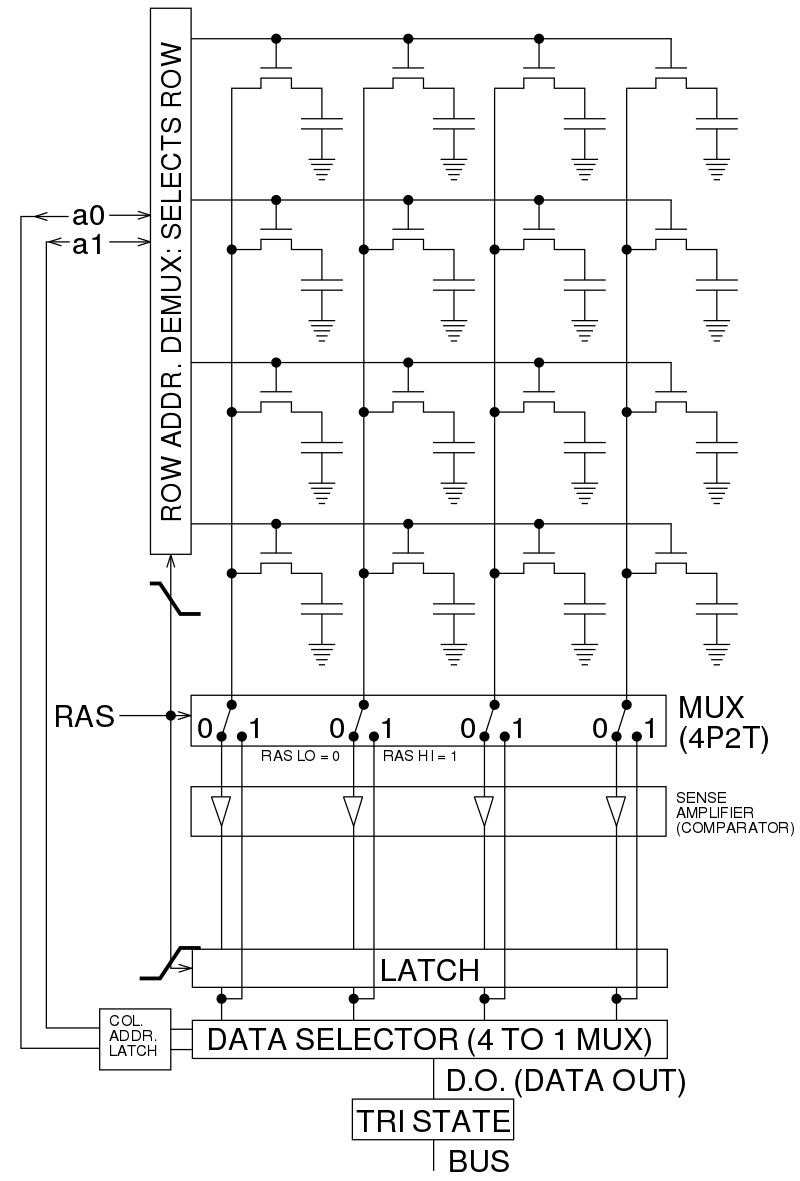
\includegraphics[width=0.35\textwidth]{Dram4x4.png}
    \caption{Array 4x4 DRAM} 
    \label{fig:DRam4x4} 
\end{figure}
\iffalse
Given a sequence of $n$ points in the plane $(X_1, Y_1), \ldots, (X_n, Y_n)$
we seek the linear equation $y = a + bx$ that approximates the points
as closely as possible, in the sense that the sum of the squared residuals
$E = \sum_{i=1}^n (Y_i - a - bX_i)^2$ is minimized.

We assume that not all of the points lie on a single horizontal or vertical
line. In that case, we can apply a \emph{transformation} to the points
so that $\sum x_i = \sum y_i = 0$ and $\sum x_i^2 = \sum y_i^2 = 1$.
The transformation is defined by
$$
x_i = \frac{X_i - \overline{X}}{\sqrt{\sum (X_i - \overline{X})^2}}\quad\text{and}\quad
y_i = \frac{Y_i - \overline{Y}}{\sqrt{\sum (Y_i - \overline{Y})^2}}.
$$

This transformation is linear, so it maps lines to lines.
If we transform a line fitted to the data,
the sum of squared residuals is multiplied by a positive constant factor.
Therefore, the transformation preserves the line of best fit.


Let $r = \sum x_i y_i$. Then
\begin{align*}
E &= \sum (y_i - a - bx_i)^2 \\
&= \sum (y_i^2 + a^2 + b^2 x_i^2 - 2ay_i - 2bx_iy_i + 2abx_i) \\
&= \sum y_i^2 + \sum a^2 + \sum b^2 x_i^2 
 - \sum 2ay_i - \sum 2bx_iy_i + \sum 2abx_i \\
&= 1 + na^2 + b^2 - 2br \\
&= (1-r^2) + na^2 + (b - r)^2\ .
\end{align*}

The sum is minimized when $a = 0$ and $b = r$, so the line of best fit is
$y = rx$. What a simple equation!
Unfortunately, the equation is a bit messier when expressed in terms of the
original variables.

\begin{align*}
\frac{y - \overline{Y}}{\sqrt{\sum (Y_i - \overline{Y})^2}}
&= \left(
     \frac{\sum (X_i - \overline{X}) (Y_i - \overline{Y})}
          {\sqrt{\sum (X_i - \overline{X})^2 \sum (Y_i - \overline{Y})^2}}
   \right)
   \left(
     \frac{x - \overline{X}}
          {\sqrt{\sum (X_i - \overline{X})^2}}
   \right)\\
y - \overline{Y} &=
\left(
     \frac{\sum (X_i - \overline{X}) (Y_i - \overline{Y})}
          {\sum (X_i - \overline{X})^2}
   \right)
   (x - \overline{X})\ .
\end{align*}

Note that $r$ is the Pearson correlation coefficient of the sample.
This shows that the correlation coefficient can be interpreted geometrically
as the slope of the line of best fit when the $x$ and $y$ values are standardized.
\fi


\section{ROM (READ ONLY MEMORY) - PROM, EPROM e EEPROM}

Começamos com as vantágens da ROM em relação à RAM:
\begin{itemize}
     \item Maior capacidade de armazenamento ;
     \item Não volatilidade: conteúdo é preservado mesmo após o desligamento do fornecimento energético;
     \item Mais rápidas;
     \item Baixo consumo energético $\rightarrow$ a ROM não consome energia para manter o seu conteúdo.
\end{itemize}

\begin{figure}[h!] 
    \centering 
    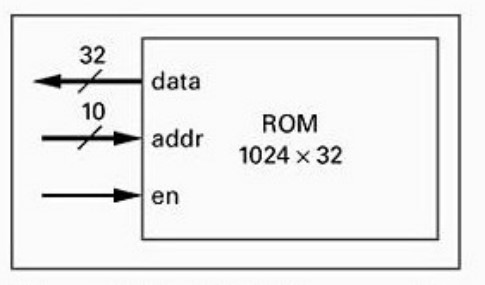
\includegraphics[width=0.35\textwidth]{simbuloROM.jpg}
    \caption{Símbulo memória ROM} 
    \label{fig:simbuloROM} 
\end{figure}

É importante notar, aqui, que não há mais entrada de dados, apenas saída, como indicado pelo símbulo e, também, não há mais clock: ROM pode ser entendida como uma unidade puramente combinacional, embora existam variações.

\begin{figure}[h!] 
    \centering 
    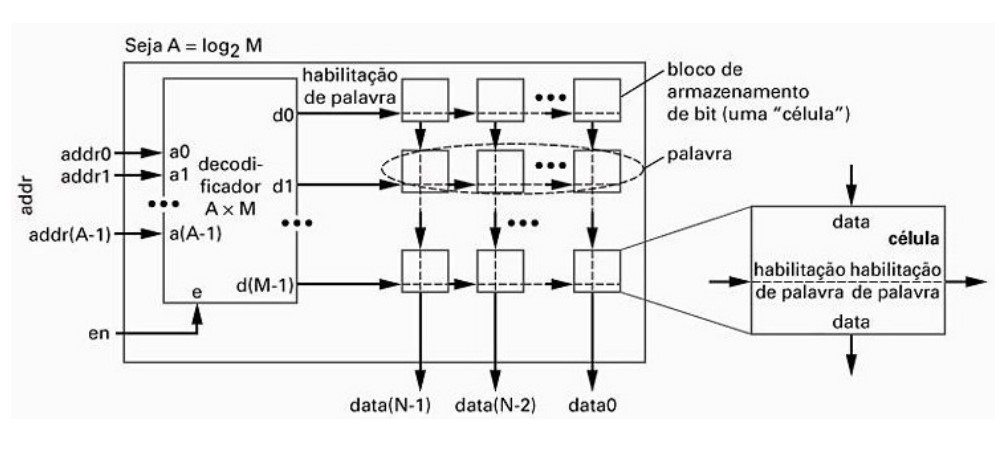
\includegraphics[width=0.7\textwidth]{estruturaRom.jpg}
    \caption{Estrutura da $ROM$, organizada em células que formam palavras na horizontal.} 
    \label{fig:estruturaRom} 
\end{figure}

 \newpage
\subsection{Programando o conteúdo da ROM}
O conteúdo sempre é programado durante a fabricação do chip, sendo as conexões feitas durante o processo.

\subsubsection{ROM programável por máscara}
ROMs programáveis por máscara são mais compactas que outros tipos de ROM. Para programar um $1$ lógico, a célula é conectada ao VCC. Para programar um $0$ lógico, a célula é conectada ao GND. Dessa forma, a programação não pode mais ser refeita.

\begin{figure}[h!] 
    \centering 
    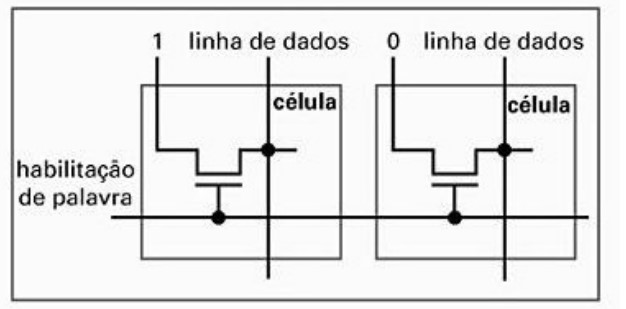
\includegraphics[width=0.5\textwidth]{programacaoRomMascara.jpg}
    \caption{ROM programada por máscara} 
    \label{fig:mascaraRom} 
\end{figure}

\newpage
\subsubsection{OTP-ROM - ROM programável por fusível - PROM}
Este tipo de ROM utiliza um fusível em cada célula, que, ao ser fabricada, possui todos os fusíveis intactos.

\begin{figure}[h!] 
    \centering 
    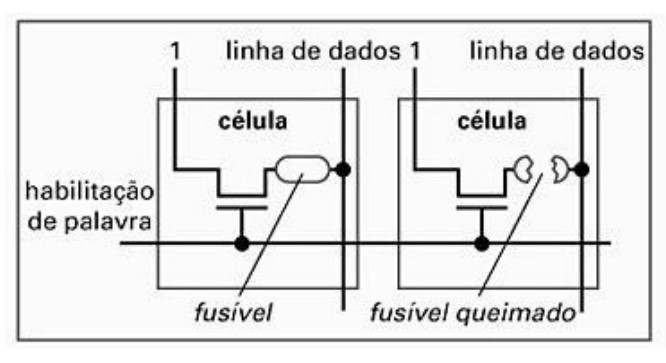
\includegraphics[width=0.5\textwidth]{programacaoPROM.jpg}
    \caption{ROM programável por fusível - OTP-ROM/PROM} 
    \label{fig:fusívelPRom} 
\end{figure}

Para programá-la, utiliza-se um dispositivo que fornece uma corrente acima do normal àquelas células que se deseja programar com $0$. Para a detecção desta alta impedância como um $0$ lógico, é utilizado um circuito extra. Esse tipo de ROM também não é reprogramável



\subsubsection{PROM apagável - Erasable PROM - EPROM}
Este tipo ROM utiliza um tipo de transistor com "porta flutuante," na qual os elétrons ficam aprisionados. Um transistor que possui elétrons aprisionados em sua porta permanece em estado de não condução, ou seja, está programado para armazenar um $0$.
Inicialmente, os transistores não possuem elétrons aprisionados, logo, estão todos em estado lógico $1$.

 
\begin{figure}[h]
\centering
\begin{minipage}{0.48\textwidth}
    \centering
    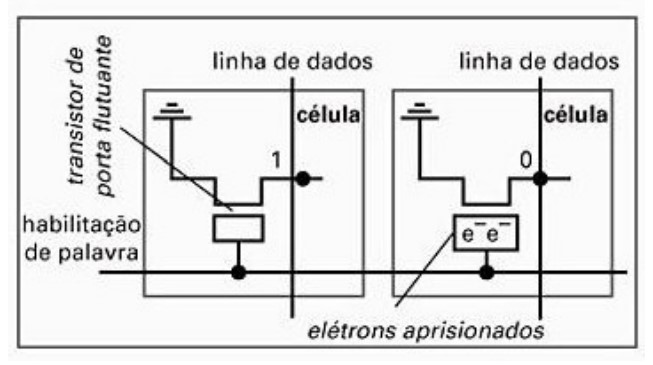
\includegraphics[width=\linewidth]{estruturaEPROM.jpg}
    \caption{PROM apagável - Erasable PROM - EPROM}
    \label{fig:EPROM}
\end{minipage}\hfill
\begin{minipage}{0.48\textwidth}
    \centering
    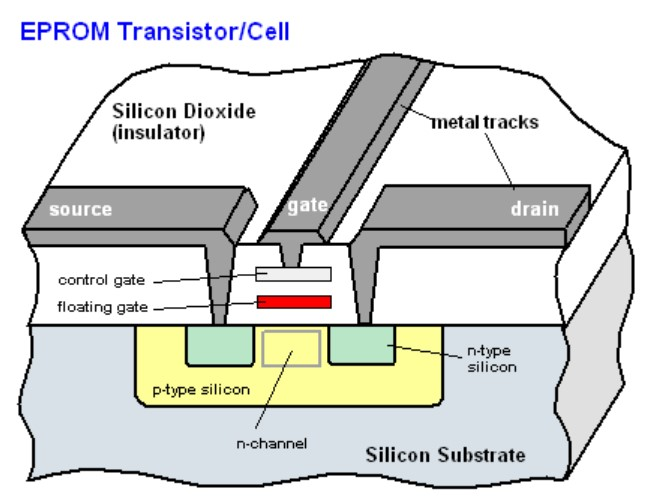
\includegraphics[width=\linewidth]{EPROMS2.jpg}
    \caption{Floating-gate MOSFET - Transistor utilizado nos EPROMS}
    \label{fig:transistorEprom}
\end{minipage}
\end{figure}

Para a programação, um dispositivo aplica uma alta tensão àqueles transistores daquelas células que devem armazenar $0$. Essa alta tensão, produz um efeito de tunelamento atráves do pequeno material isolante até a porta flutuante, fazendo os elétrons acumulares. Quando a tensão é removida, os elétrons não tem energia suficiente para criar o túnel de volta, permanecendo aprisionados na célula. Como consequencia, há o aumento da tensão de threshold para o transistor fechar o canal.

Para que o conteúdo seja apagado, o chip da placa de circuito da EPROM precisa ser retirado e exposto à luz ultravioleta para energizar os elétrons aprisionados previamente, de forma que possam vencer a barreira do material isolante da porta flutuante, apagando, assim, todos os $0$'s. É importante mencionar que \textbf{todo} o conteúdo é apagado: não é possível apagar somente uma parte da memória. Em média, podem ser apagadas e reprogramadas mais de 10 mil vezes, mantendo o conteúdo por 10 anos ou mais.

\begin{figure}[h!] 
    \centering 
    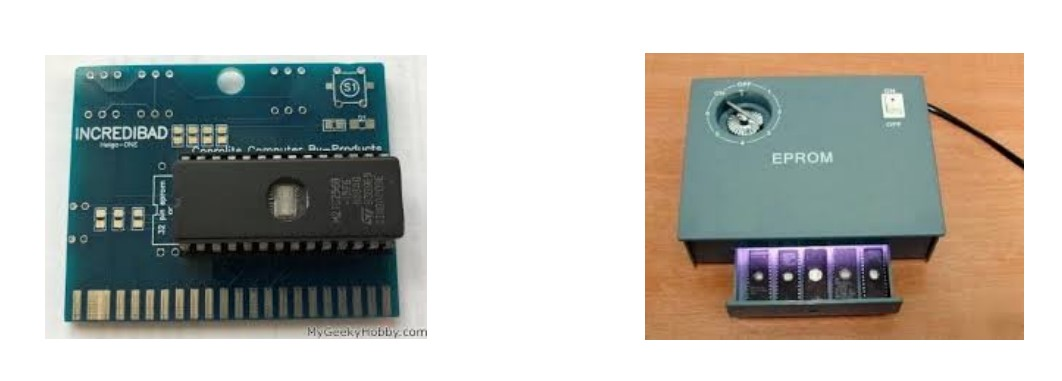
\includegraphics[width=1\textwidth]{EPROMS.jpg}
    \caption{Chips EPROMs expostos.} 
    \label{fig:EPROMExposto} 
\end{figure}

\subsubsection{PROM eletricamente apagável - EEPROM}
A diferença base entre uma EPROM e uma EEPROM é que esta não precisa de luz UV para ser apagada e sim de uma alta tensão na linha de dados. Também, aqui, essa tensão pode ser aplicada em células específicas, ou seja, é possível apagar e reprogramar apenas certas palavras.
\begin{figure}[h!] 
    \centering 
    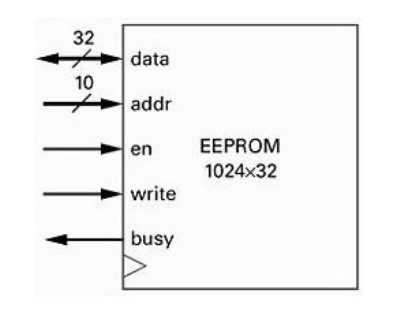
\includegraphics[width=0.5\textwidth]{EEPROM.jpg}
    \caption{Símbulo memória EEPROM} 
    \label{fig:EEProm} 
\end{figure}



A estrutura base de uma memória EEPROM é vista na imagem \ref{fig:EEPromStructure}. Aqui, são utilizados dois transistores, sendo um deles um \textit{Floating-gate MOSFET}, do mesmo tipo utilizado nas EPROMS. O MOSFET tradicional é utilizado para selecionar qual célula deseja escrever; já o FGMOS contem o valor guardado na célula.

\begin{figure}[h!] 
    \centering 
    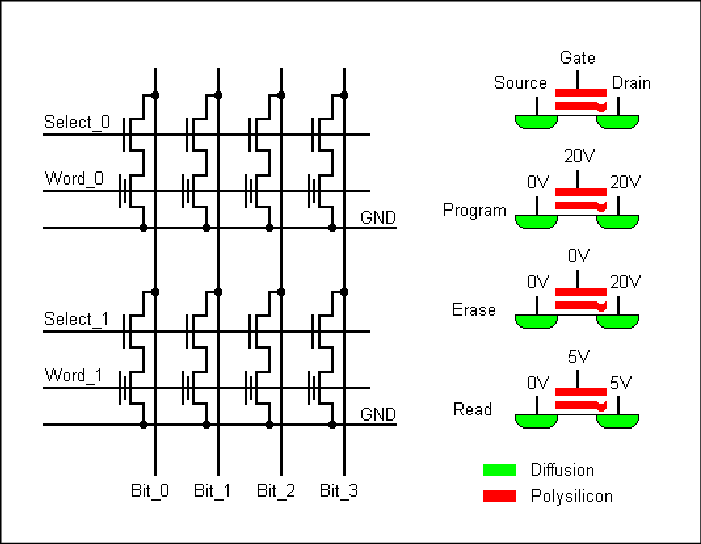
\includegraphics[width=0.8\textwidth]{eepromgood.png}
    \caption{Estrutura de um array de memorias EEPROM.} 
    \label{fig:EEPromStructure} 
\end{figure}

Para se escrever em uma célula, aplica-se tensões altas no gate e drain do FGMOS, causando assim o tunelamento e, assim, o aprisionamento dos elétrons na porta flutuante.

Para apagar o valor em uma célula, aplica-se uma alta tensão no drain do FGMOS, concedendo energia suficiente para os elétrons presos na porta flutuante para saírem pela porta drain e assim apagar o valor guardado no transistor.

\begin{figure}[!h]
\centering
\begin{minipage}{0.38\textwidth}
    \centering
    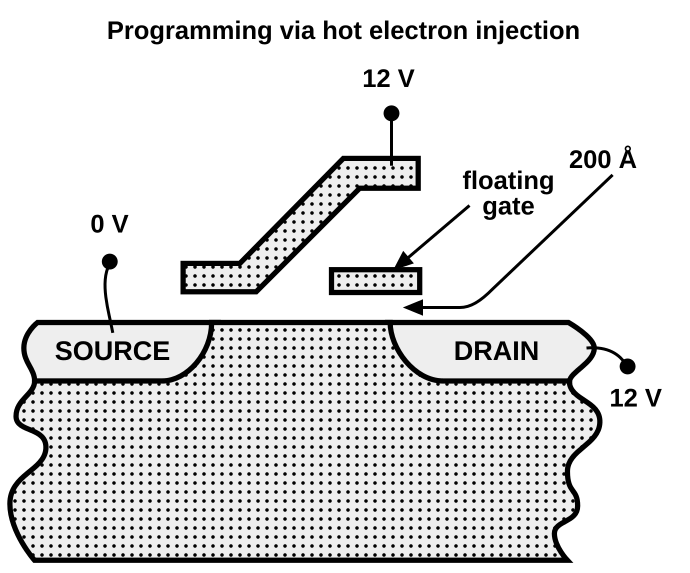
\includegraphics[width=\linewidth]{CharginEEPROM.png}
    \caption{Escrevendo em uma unidade EEPROM}
    \label{fig:writingEEPROM}
\end{minipage}\hfill
\begin{minipage}{0.38\textwidth}
    \centering
    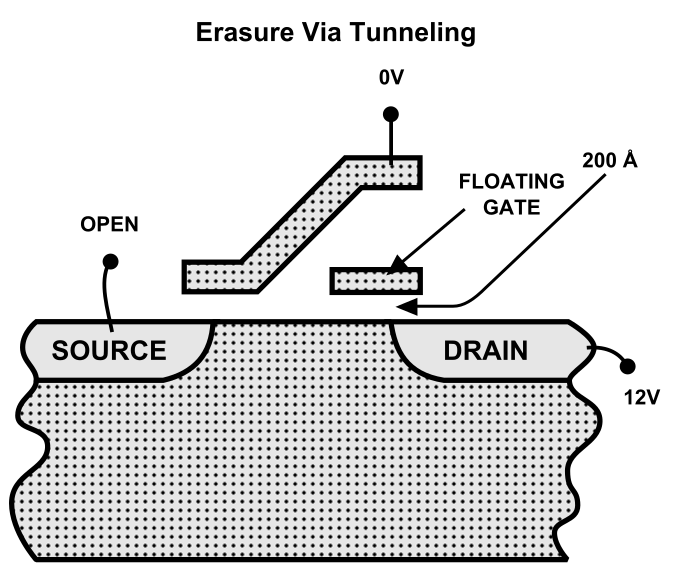
\includegraphics[width=\linewidth]{DischarginEEPROM.png}
    \caption{Apagando em uma unidade EEPROM}
    \label{fig:dischargingEEPROM}
\end{minipage}
\end{figure}

Memórias EEPROM modernas(\textit{in system programmable(ISP)}) possuem controladores internos para programação, ou seja, é possível programa o conteúdo de uma EEPROM sem retirar o chip da placa de circuito. Ou seja, funcionam de forma similar a uma RAM. Contudo, a programação de uma EEPROM leva muito mais tempo do que a leitura, uma sendo da ordem de dezenas de microssegundos e a outra da ordem de nanossegundos, respectivamente. EEPROMs podem ser programadas milhões de vezes e preservar seu conteúdo por cem anos ou mais sem energia. 

Embora as EEPROMs permitam apagar célular individuais, existem aplicações nas quais é necessário apagar grandes blocos de memória. Neste caso, são utilizadas as memórias Flash, que implementam justamente essa funcionalidade. Ou seja, memórias Flash não são apagáveis por bit(ou \textit{bit erasable}), mas sim apagáveis globalmente. Também, as células podem ser de apenas um transistor, aumentando a densidade de componentes se comparado com memórias EEPROM.


\end{document}


